\subsection{Besturingssysteemsoftware}

Het ontwerp van het geheugenbeheer van een OS is afhankelijk van 3 fundamentele keuzes:

\begin{itemize}
\item Gebruik van virtueel geheugen?
\item Pagineren, segmenteren of beide?
\item Kiezen van algoritmes die worden toegepast voor allerlei aspecten van het geheugenbeheer
\end{itemize}

\begingroup
\setlength{\tabcolsep}{10pt} % Default value: 6pt
\renewcommand{\arraystretch}{1.5} % Default value: 1
\begin{table}[hp]
\begin{center}
  \begin{tabular}{| p{8cm} | p{8cm} | }
    \hline %rij 1
\textbf{Ophaalstrategie} 
\begin{itemize}
\item Vraag
\item Herpagineren
\end{itemize} & \textbf{Beheer residente set}
\begin{itemize}
    \item Grootte residente set
        \begin{itemize}
            \item vast
            \item variabel
        \end{itemize}
    \item vervangingsbereik
        \begin{itemize}
            \item globaal 
            \item lokaal
        \end{itemize}
\end{itemize}  \\ \hline
%rij2
\textbf{Plaatsingsstrategie}
& \textbf{Opschoonstrategie}
\begin{itemize}
    \item vraag
    \item vooral opschonen
\end{itemize}  \\ \hline
%rij3
\textbf{Vervangingsstrategie}
\begin{itemize}
    \item optimaal
    \item Least Recently Used (LRU)
    \item First in First Out
    \item Klok
    \item Paginabuffering
\end{itemize} 
& \textbf{Beheer van procesbelasting}
\begin{itemize}
    \item Multiprogrammeringsgraad
\end{itemize}  \\
    \hline
  \end{tabular}
\end{center}
\caption{}
\label{}
\end{table}
\endgroup

\subsubsection{Strategie bij ophalen (fetch policy )}

Deze strategie bepaalt wanneer een pagina moet worden overgebracht naar het hoofdgeheugen. Twee types:

\begin{itemize}
    \item Vraagpaginering (demand paging)
        \begin{itemize}
        \item Laadt enkel pagina’s in het hoofdgeheugen wanneer een referentie is gemaakt naar de locatie op de pagina
        \item Veel paginafouten wanneer het proces eerst wordt gestart
        \end{itemize}
    \item Prepaginering (prepaging)
    \begin{itemize}
        \item Laadt meer pagina’s in dan nodig
        \item Meer efficiënt om pagina’s in te halen die elkaar opvolgen in het geheugen
        \item Niet verwarren met swapping!
        \end{itemize}

\end{itemize}


\subsubsection{Strategie bij plaatsing}

Deze strategie bepaalt waar een stuk van het proces terechtkomt in het geheugen. best-fit, first-fit, ... Belangrijk bij segmentering.

Bij zuiver pagineren of een combinatie van segmentering en paginering maakt deze strategie niets uit omdat de hardware voor de adresvertaling en de hardware voor geheugentoegang even efficiënt kunnen werken voor elke pagina/framecombinatie.


\subsubsection{Strategie bij vervanging}

Wanneer alle frames in het hoofdgeheugen in gebruik zijn en het belangrijk is om een nieuwe pagina in te laden, bepaalt de vervangingsstrategie welke pagina in het hoofdgeheugen vervangen moet worden.

Maar, welke pagina wordt er dan verplaatst?

De pagina die dan verplaatst wordt moet de pagina zijn de het minst waarschijnlijk gebruikt ga worden in de nabije toekomst. Dat wordt bepaald door het principe van lokaliteit.

Meeste strategieën worden bepaald op basis van het oude gedrag.

\textbf{Framevergrendeling:}

Wanneer een frame vergrendeld is (grendelbit staat op 1 in de frame- of de paginatabel) => pagina kan niet worden verwijderd in het hoofdgeheugen om te worden vervangen.


\textbf{Elementaire algoritmen:}

\begin{itemize}
\item Optimaal: vervangt de pagina waarnaar het verst in de toekomst gerefereerd zal worden. Dit is echter puur theoretisch omdat dit van het OS vereist dat het op de hoogte is van alle toekomstige referenties.
\item Least recently used (LRU): vervang de pagina waarnaar het minst recent is gerefereerd: volgens beginsel van lokaliteit is dit de pagina met de kleinste kans om in de toekomst naar gerefereerd te worden.
\item FIFO: pagina's worden om beurten verwijderd (round robin) => de pagina die het langst in het geheugen is wordt vervangen. Dit is nadelig want het zou kunnen zijn dat die in de nabije toekomst weer nodig is => paginafout. Maar, het voordeel is dat dit gemakkelijk te implementeren is.
\item Klok: aan elk frame wordt een extra bit toegevoegd: de u(se)-bit. Wanneer een pagina voor het eerst in het geheugen wordt geladen, dan wordt de pointer naar het volgende frame gezet. Als naar de pagina verwezen wordt, dan wordt de use bit op 1 gezet. Wanneer een pagina vervangen moet worden, dan wordt het eerste frame dat tegengekomen wordt met een use bit op 0 vervangen. Tijdens het zoeken voor vervanging wordt elke use bit die op 1 staat, op 0 gezet (zie fig 8-15)
\end{itemize}

Het verschil met FIFO is dat sommige frames (met u-bit==1) worden overgeslagen en dat het niet altijd de oudste pagina moet zijn die vervangen wordt.

\textbf{Men heeft gevonden dat, naarmate er meer frames worden toegewezen aan een proces, het verschil in paginafouten kleiner en kleiner wordt tussen de verschillende strategieën => kan het lonen om te opteren voor een simpele strategie omdat deze minder tijd in beslag neemt om uit te voeren.}

Het klokalgoritme kan krachtiger worden gemaakt door het aantal bits te verhogen. En ook tweede bit naast de u-bit: de m-bit => 4 categorieën:

\begin{itemize}
\item geen recente toegang, ongewijzigd (u:0;m:0)
\item recente toegang, ongewijzigd (u:1;m:0)
\item geen recente toegang, gewijzigd (u:0;m:1)
\item recente toegang, gewijzigd (u:1;m:1)
\end{itemize}

\textbf{Het klokalgoritme werkt dan zo:}

\begin{enumerate}
\item zoek naar frames waarbij u==0 en m==0; het eerste frame dat hieraan voldoet wordt vervangen;
\item mislukt dat, dan wordt het eerste frame met u==0 en m==1 vervangen;
\item mislukt ook dat, dan gaan we nog eens door de frames want nu zijn alle u-bits die daarvoor 1 waren 0 geworden en is er dus zeker 1 frame dat voldoet aan u==0;m==0 OF u==0;m==1
\end{enumerate}

Waarom u==0 en m==1 als tweede keuze: omdat dit frame niet recent is gebruikt en dus is de kans dat het binnenkort opnieuw gaat moeten gebruikt worden klein. Het frame moet wel weggeschreven worden voordat het wordt vervangen maar dat weegt op tegen het feit dat het misschien niet nodig is in de toekomst.


\begin{figure}[htp]
    \centering
            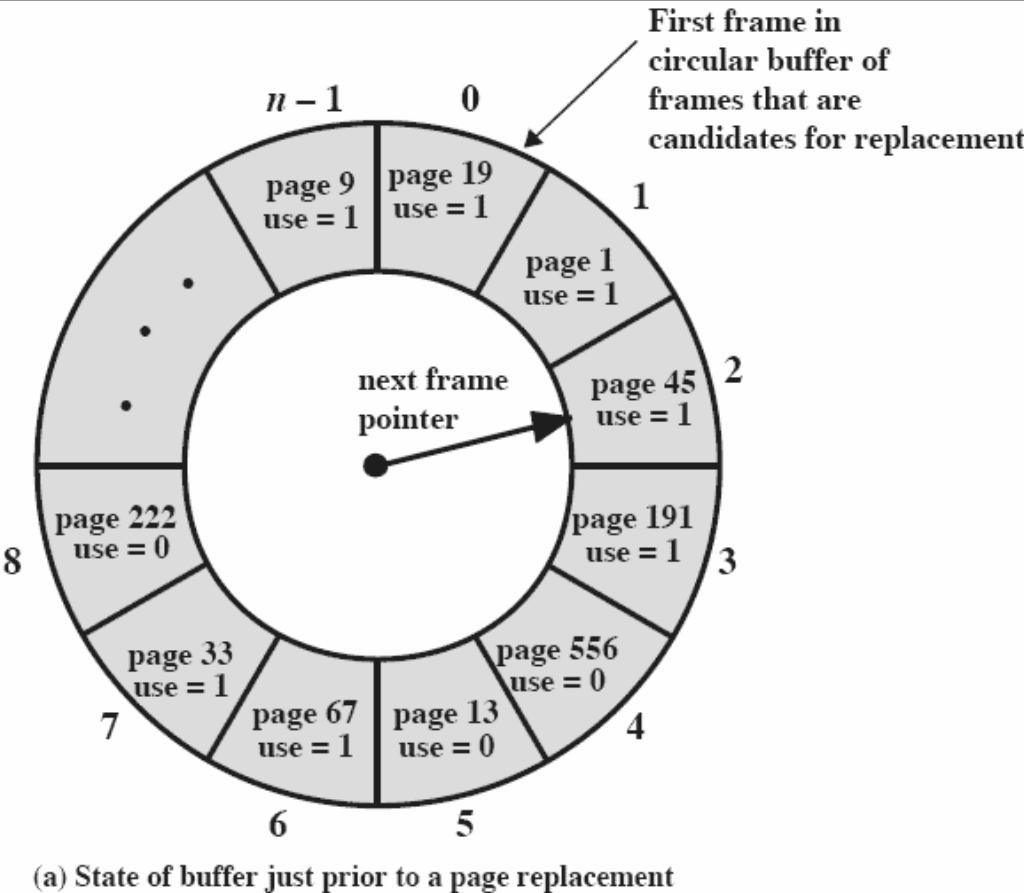
\includegraphics[width=4in]{img/klok1}
        \caption{}
    \label{fig:}
\end{figure}

\begin{figure}[htp]
    \centering
            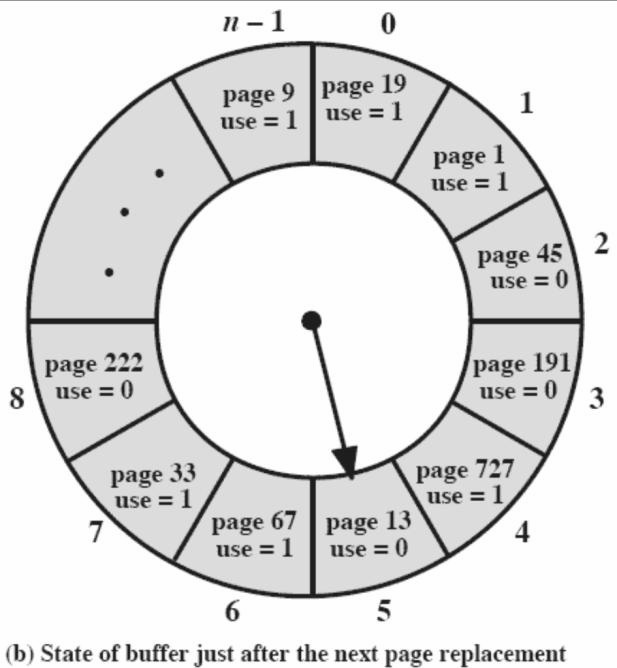
\includegraphics[width=4in]{img/klok2}
        \caption{}
    \label{fig:}
\end{figure}

\begin{figure}[htp]
    \centering
            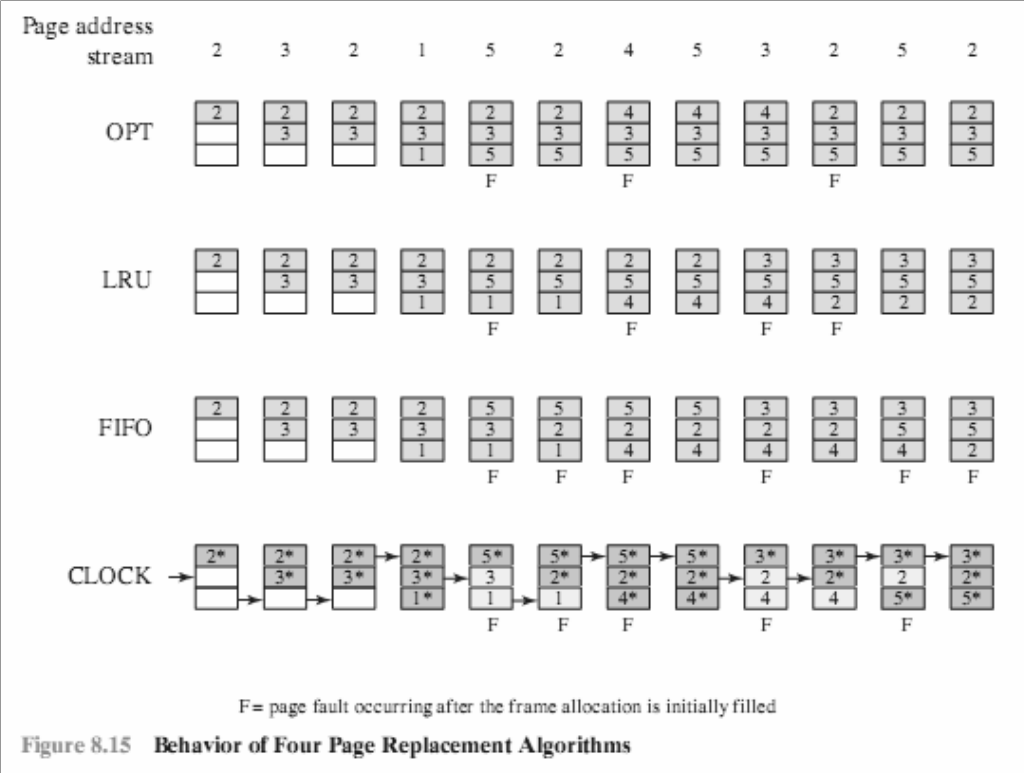
\includegraphics[width=4in]{img/pagereplacementalgoritm}
        \caption{}
    \label{fig:}
\end{figure}



\textbf{Paginabuffering}

LRU en klok zijn superieur aan FIFO MAAR complexer en meer overhead. De kosten van vervanging van een gewijzigde pagina zijn groter dan die van een ongewijzigde pagina.

Oplossing is dat de vervangende pagina toegevoegd kan worden naar een van twee lijsten:

\begin{itemize}
\item Lijst met vrije pagina’s die nog niet gewijzigd zijn.
\item Lijst met pagina’s die gewijzigd zijn.
\end{itemize}

De pagina wordt niet verwijderd uit het hoofdgeheugen maar de PTE wordt verwijderd uit de paginatabel en in de juiste lijst (vrije/gewijzigde) geplaatst.

VOORDELEN paginabuffering:


\begin{itemize}
\item Het kost weinig om de pagina terug in te laden in de residente set, gewoon de PTE uit de lijst halen en in de paginatabel zetten.
\item Gewijzigde pagina's worden weggeschreven in clusters, niet 1 per 1, dat vermindert het aantal I/O bewerkingen en daarmee ook de schijftoegangstijd.
\end{itemize}


Paginabuffering werkt dan als een soort van cache voor pagina's.


\subsubsection{Beheer van de residente set}

Het besturingssysteem moet beslissen hoeveel pagina’s moeten ingeladen worden in het hoofdgeheugen.

\begin{itemize}
\item Hoe kleiner de hoeveelheid geheugen is die wordt toegewezen aan enen proces, des te groter het aantal processen dat zich in het geheugen kunnen bevinden.
\item Kleine aantallen van pagina’s ingeladen, vergroot het aantal paginafouten.
\item Vanaf een bepaalde grootte heeft een extra toewijzing van hoofdgeheugen aan een proces geen effect meer op de foutfrequentie vanwege het lokaliteitsprincipe.
\end{itemize}

\textbf{Grootte van de residente set}

\begin{itemize}
\item Vaste toewijzing: een proces krijgt een vast aantal pagina's waarbinnen het moet worden uitgevoerd; dat aantal wordt bepaald bij de eerste keer dat het proces geladen wordt. Wanneer tijdens de verwerking een paginafout optreedt, dan moet een procespagina vervangen worden door een nieuw aangevraagde pagina
\item Variabele toewijzing: het aantal frames dat is toegewezen aan een proces kan variëren gedurende de levensloop van het proces. Een proces dat veel paginafouten genereert geeft aan dat het beginsel van lokaliteit slechts in beperkte mate geldt voor dat proces. Dan kan het aantal toegewezen frames aangepast(verhoogd) worden. Omgekeerd kan ook, als er zeer weinig paginafouten gegenereerd worden, dan kunnen er gerust minder frames worden toegewezen. Variabele toewijzing hangt samen met het concept 'Vervangingsbereik'
\end{itemize}

\newpage
\begin{landscape}

\textbf{Vervangingsbereik}

Het bereik van een vervangingsstrategie kan opgedeeld worden in twee categorieën: globaal of lokaal. Beide types worden geactiveerd bij een paginafout wanneer er geen vrije pagina frames meer zijn.

Een lokale vervanging kiest tussen alle residente pagina’s van het process.

Een globale vervanging kiest tussen alle niet geblokkeerde pagina’s in het hoofdgeheugen.

Het vervangingsbereik hangt samen met de grootte van de residente set:

\begin{table}[ht]
\begin{center}
\begin{tabular}{|c|p{8cm}|p{8cm}|}
\cline{2-3}
\multicolumn{1}{c|}{} & lokale vervanging & globale vervanging \\
\hline
vaste toewijzing & \begin{itemize}
\item het aantal aan een proces toegewezen frames ligt vast

\item de te vervangen pagina wordt gekozen uit de frames die zijn toegewezen aan het proces
\end{itemize}
& gaat niet: om de grootte van de residente set gelijk te houden moet een pagina van de residente set vervangen worden door een andere pagina van de residente set \\
\hline
variabele toewijzing & \begin{itemize}
\item het aantal toegewezen frames kan wijzigen voor het behoud van de werkset (working set) van het proces

\item de te vervangen pagina wordt gekozen uit de frames die zijn toegewezen aan het proces
\end{itemize} &  de te vervangen pagina's worden gekozen uit alle beschikbare (niet- vergrendelde) frames in het hoofdgeheugen => de grootte van de residente set kan variëren \\
\hline
\end{tabular}
\end{center}
\caption{Table caption.}
\label{Table1}
\end{table}

\end{landscape}

\textbf{Vaste toewijzing met lokaal bereik}

\begin{itemize}
    \item proces wordt uitgevoerd in hoofdgeheugen met vast aantal pagina's
    \item paginafout => welke pagina v.d. residente set gaat vervangen worden?
    \item van tevoren moet worden beslist hoeveel ruimte wordt toegewezen aan een proces; nadelen:
        \begin{itemize}
        \item als dit te weinig is: paginafouten
        \item te veel: er kunnen te weinig processen ingeladen worden in het hoofdgeheugen => er wordt veel tijd besteed aan het swappen van processen
        \end{itemize}
\end{itemize}

Variabele toewijzing met globaal bereik

\begin{itemize}
\item gemakkelijkste vorm om te implementeren.
\item paginafout => vrij frame toevoegen aan de frames die zijn toegewezen aan het proces en de pagina daaraan toewijzen.
\item zijn er geen vrije frames meer, dan wordt een pagina vervangen van om het even welk proces. De moeilijkheid is deze keuze maken. Dit kan verholpen worden door gebruikt te maken van paginabuffering omdat een pagina opnieuw kan worden gebruikt als die nog niet is weggeschreven naar de harde schijf.
\end{itemize}




\textbf{Variabele toewijzing met lokaal bereik}

Probeert de problemen die ontstaan door het werken met globaal bereik te omzeilen:

\begin{itemize}
\item wordt een nieuw proces in het hoofdgeheugen geladen, wijs daar dan een bepaald aantal frames aan toe en gebruik prepaginering of vraagpaginering voor het vullen van de rest van de toewijzing.
\item paginafout => selecteer de te vervangen pagina uit de residente set van het proces dat de fout heeft veroorzaakt.
\item evalueer de toewijzing aan het proces zo nu en dan en verhoog of verlaag het aantal toegewezen frames indien nodig.
\end{itemize}
Een veelbesproken methode: de \textbf{werksetbenadering}.

werkset = een verzameling pagina's van een proces waarnaar verwezen is binnen een bepaald tijdsvenster

=> als tijdsvenster groter wordt, dan wordt de werkset groter.

De werkset hangt nauw samen met lokaliteit: door dat beginsel gebruikt het proces een stabiele set aan pagina's waarvan de inhoud van de werkset slechts minimaal verandert, volgende overgangsperioden wijzen op een verandering naar een nieuwe lokaliteit.


Tijdens een overgangsfase blijven een aantal pagina's uit de oude lokaliteit binnen het venster wat leidt tot een forse toename van de grootte van de werkset bij verwijzingen naar nieuwe pagina's. Verschuift het venster over deze paginaverwijzingen, dan neemt de werksetgrootte af totdat de werkset uitsluitend pagina's bevat die behoren tot de nieuwe lokaliteit.

Werkset kan worden gebruikt als leidraad bij een strategie voor de grootte van de residente set:

\begin{itemize}
\item controleer de grootte van de werkset van elk proces
\item verwijder regelmatig pagina's uit de residente set van een proces die niet voorkomen in de residente set van een proces (vergelijkbaar met LRU)
\item een proces mag alleen worden uitgevoerd als zijn werkset zich in het hoofdgeheugen bevindt = als zijn residente set zijn werkset bevat => minder initiële paginafouten
\end{itemize}

Beperkingen van de werksetbenadering:

\begin{itemize}
\item de toekomst kan niet worden voorspeld op basis van het verleden; zowel de grootte als de samenstelling van de werkset zullen na verloop van tijd veranderen
\item het nauwkeurig meten van de werkset van ieder proces is onpraktisch want dit vereist een timestamp voor iedere paginaverwijzing van elk proces = nogal veel
\item optimale waarde van is onbekend en zal wisselen
\end{itemize}

\textbf{desalniettemin is de gedachte goed en daarom zijn er een aantal OS'en die het trachten te implementeren}

\subsubsection{Opschoon strategie}

Een opschoonstrategie bepaalt wanneer een gewijzigde pagina moet worden weggeschreven naar het secundaire geheugen.

Twee mogelijkheden:

\begin{itemize}
\item Vraagopschoning : een pagina wordt alleen weggeschreven wanneer die geselecteerd is voor vervanging.
\item Precleaning:  gewijzigde pagina's worden weggeschreven voordat hun frames nodig zijn. Pagina’s kunnen in batches worden weggeschreven.
\end{itemize}

Nadelen:

\begin{itemize}
\item Vraagopschoning: het schrijven van een vervuilde pagina moet gekoppeld zijn aan het inlezen van een nieuwe pagina. Het processorgebruik kan afnemen omdat het proces dat de paginafout veroorzaakte moet wachten op twee paginaoverdrachten.
\item Precleaning: de overdrachtscapaciteit van het secundair geheugen is beperkt en mag niet worden verspild aan onnodig wegschrijven en het wegschrijven van een pagina die toch in het hoofdgeheugen blijft en nog eens gewijzigd wordt, dat is een onnodige schrijfbewerking geweest.
\end{itemize}	

De betere benadering gebruikt page buffering. Hierbij worden de pagina’s in twee lijsten geplaatst: gewijzigd en ongewijzigd.

Pagina’s in de gewijzigde lijst worden tijdelijk uitgeschreven in batches.

Pagina’s in de ongewijzigde lijst worden teruggehaald wanneer er wordt naar gerefereerd of gaat verloren wanneer het oorspronkelijk frame van de pagina wordt toegewezen aan een andere pagina.

\subsubsection{Toezicht op de procesbelasting}

Dit bepaalt het nummer van processen dat resident kan zijn in het hoofdgeheugen, dit is het niveau van multiprogramming.

Bij te weinig processen en alle processen geblokkeerd, zal er veel tijd worden gespendeerd aan \textbf{swappen}. Als er teveel processen worden toegelaten kan dit lijden tot \textbf{trashing}.

\textbf{Niveau van multiprogrammering}


\begin{figure}[htp]
    \centering
            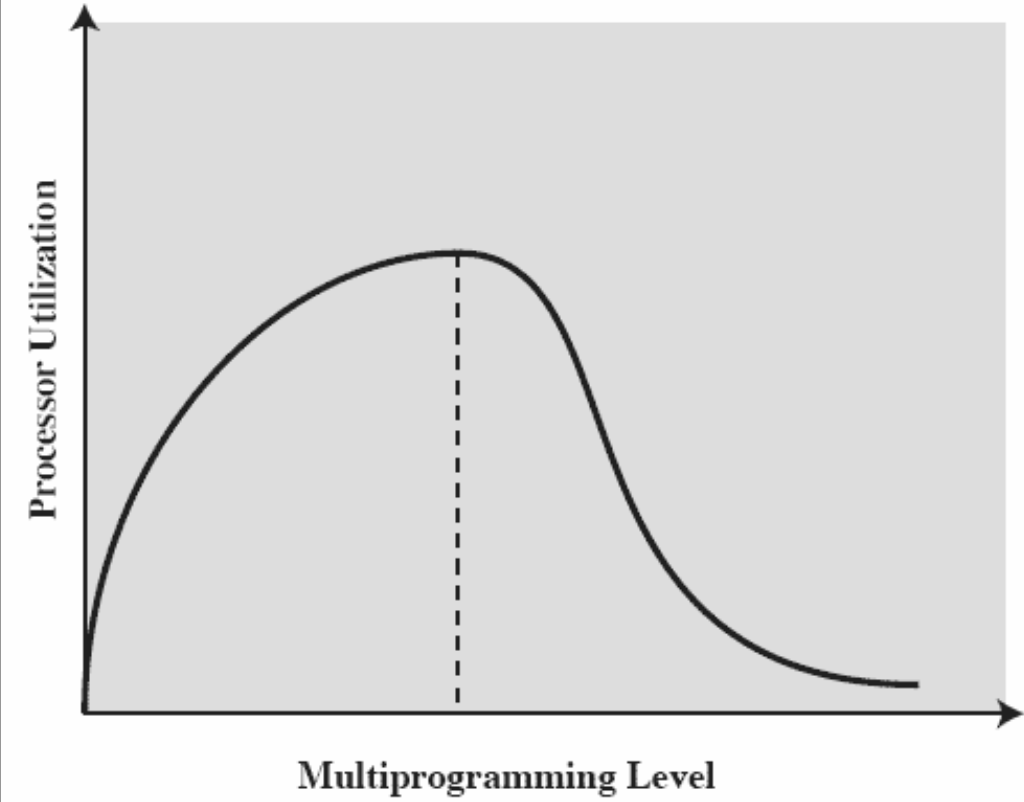
\includegraphics[width=4in]{img/procesbelasting}
        \caption{}
    \label{fig:}
\end{figure}

De afbeelding spreekt voor zichzelf, hoe meer processen worden toegelaten hoe minder de processor nuttig wordt gebruikt, zelfde moest men te weinig processen toelaten in het hoofdgeheugen.


\textbf{Opschorten van processen}

Wanneer het niveau van multiprogrammering worden verlaagd, dan moet één of meer van de residente processen worden opgeschort (uit het hoofdgeheugen worden weggeswapt); zes mogelijkheden:

\begin{itemize}
\item Proces met de laagste prioriteit
\item Proces dat een paginafout veroorzaakt: er is een grotere kans dat de werkset van dit proces niet resident is => de prestaties zullen het minst lijden onder het opschorten van dit proces
\item Laatst geactiveerd proces: hierbij is de kans het grootst dat het geen residente werkset heeft
\item Proces met de kleinste residente werkset: dit vereist de kleinste toekomstige inspanning om het proces weer te laden. Het is echter nadelig voor programma's met een beperkte lokaliteit
\item Grootste proces => bij een overvol geheugen ontstaan hierdoor de meeste vrije frames waardoor extra deactiveringen in de nabije toekomst onwaarschijnlijk maakt
\item Proces met de grootste resterende uitvoeringstijd: dit neemt immers ook plaats in aangezien het nog even kan duren vooraleer het uit het hoofdgeheugen is verdwenen wanneer het volledig is uitgevoerd
\end{itemize}